\documentclass[xelatex,ja=standard,jafont=noto]{bxjsarticle}
\usepackage[utf8]{inputenc}

\usepackage{amsmath}
\usepackage{amsthm}
\usepackage{amssymb}
\usepackage{mathrsfs}
\usepackage{graphicx} 

\usepackage{tikz}
\usetikzlibrary{shapes,arrows}
\usepackage{verbatim}
\tikzstyle{block} = [draw, fill=white, rectangle, 
    minimum height=3em, minimum width=6em]
\tikzstyle{sum} = [draw, fill=white, circle, node distance=1cm]
\tikzstyle{input} = [coordinate]
\tikzstyle{output} = [coordinate]
\tikzstyle{pinstyle} = [pin edge={to-,thin,black}]



\newtheorem{theorem}{Theorem}
\newtheorem{corollary}{Corollary}
\newtheorem{lemma}{Lemma}
\newtheorem{example}{Ex\documentclass{article}
	\usepackage{CJKutf8}
	\usepackage{amsmath}
	\usepackage{amsthm}
	\usepackage{amssymb}
	ample}
\newtheorem{definition}{Definition}

\def\ds{\displaystyle}
\def\ul{\underline}
	\title{計測制御演習課題1	}
	\author{BQ18026,関宇 }
	\date{Oct.6,2020}
	
	
\begin{document}
		\maketitle
		
		
		
	\section{物体の表面温度を$ \theta(t)$,雰囲気温度を$ \theta_{ex}(t) $ とするとき,$ \theta$の時間変化率は両者の温度差に比例することが知られている(Newtonの冷却則).この比例定数を k とする.このとき}
	
(1) 表面温度θ(t) についての微分方程式を求めよ.

\begin{equation}
	\dot{\theta(t)}=k(\theta_{ex}-\theta(t))
\end{equation}
	
	(2) $ \theta_{ex}(t)$から$ \theta(t)$に至る伝達関数を求めよ.\\
	
まず,両辺をラプラス変換を取る

\begin{equation}
	s\Theta(s)-\theta(0)=k\theta_{ex}-k\Theta(s)
\end{equation}

\begin{equation}
	(s+k)\Theta(s)=\Theta_{ex}+\theta(0)
\end{equation}

\begin{equation}
	G(s)=\frac{Y(s)}{U(s)}=\frac{k}{k+s}
\end{equation}

(3) 状態空間表現を求めよ.\\

$ x_{1}(t)=\theta(t),x_{2}(t)=\dot{\theta}(t) $とする.

\begin{equation}
\left\{
             \begin{array}{lr}
             \dot{x_{1}}(t)=k\theta_{ex}-kx_{1}(t), & \\
             &\\
             \dot{x_{2}}(t)=-kx_{2}(t), & 
             \end{array}
\right.
\end{equation}

\begin{equation}
    {
\left[ \begin{array}{c}
\dot{x_{1}}(t)\\
\dot{x_{2}}(t)
\end{array}
\right ]}={
\left[ \begin{array}{cc}
-k&0\\
0&-k
\end{array}
\right ]}{
\left[ \begin{array}{c}
x_{1}(t)\\
x_{2}(t)
\end{array}
\right ]}
+{
\left[ \begin{array}{c}
k\\
0
\end{array}
\right ]}\theta_{ex}
\end{equation}

よって、状態空間表現は

\begin{equation}
\left\{
             \begin{array}{lr}
             \dot{x}(t)=Ax(t)+Bu(t), & \\
             &\\
             y(t)=Cx(t), & 
             \end{array}
\right.
\end{equation}
特に、

\begin{equation}
A={
\left[ \begin{array}{cc}
-k&0\\
0&-k
\end{array}
\right ]},B={
\left[ \begin{array}{c}
k\\
0
\end{array}
\right ]},c=[1,0]
\end{equation}\\

(4).$ \kappa=2\times 10^{-3} $,初期条件を$ \theta(0)=300K $として,雰囲気
温度が「300+各自の学生番号の下2桁」K のときの
5分後における物体の表面温度を求めよ.\\

雰囲気温度が326K,時定数t=500s、Simulinkでシミュレーションした結果より、

\begin{figure}[h!]
    \centering
    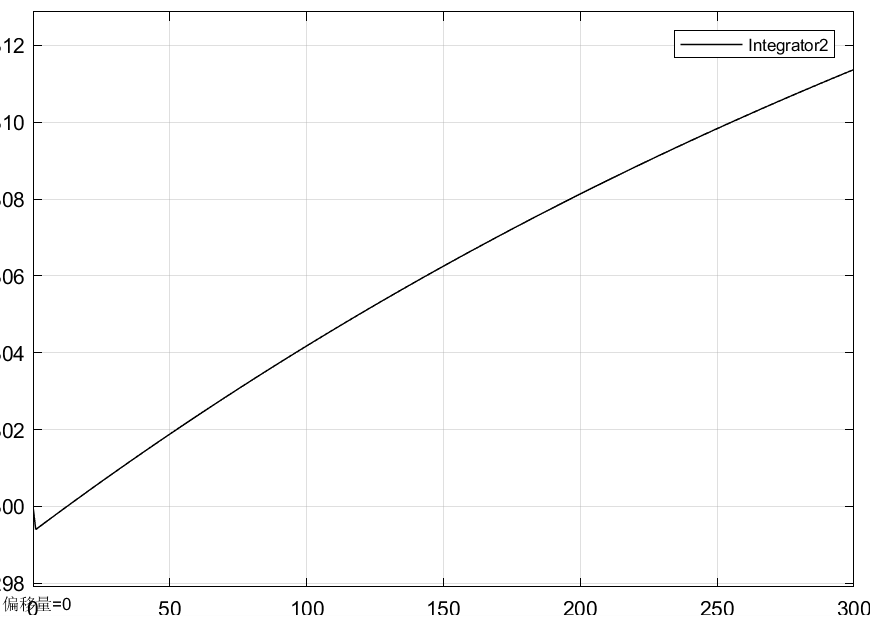
\includegraphics[scale=0.4]{01.png}
    \caption{物体の表面温度変化 }
\end{figure}

5分後における物体の表面温度は約311Kである.


\section{あるメーカの人工心臓の駆動入力電圧v(t) と血液圧送量q(t) の動特性は,以下の微分方程式で与えられている.}
	
		\begin{equation}
	\ddot{q}(t)+2\dot{q}(t)+2q(t)=v(t)
	\end{equation}
	
	(1) 血液圧送量と入力電圧についての伝達関数を求めよ.\\
	
	まず,両辺をラプラス変換を取る
	
		\begin{equation}
s^{2}Q(s)+2sQ(s)+2Q(s)=V(s)
	\end{equation}
	
	\begin{equation}
	G(s)=\frac{Y(s)}{U(s)}=\frac{1}{s^{2}+2s+2}
\end{equation}


(2) この人工心臓は,ステップ入力に関してどのような挙動を示すかを言葉で述べよ.
それは上記の動特性のどこから読み取れるか.\\

\begin{figure}[h!]
    \centering
    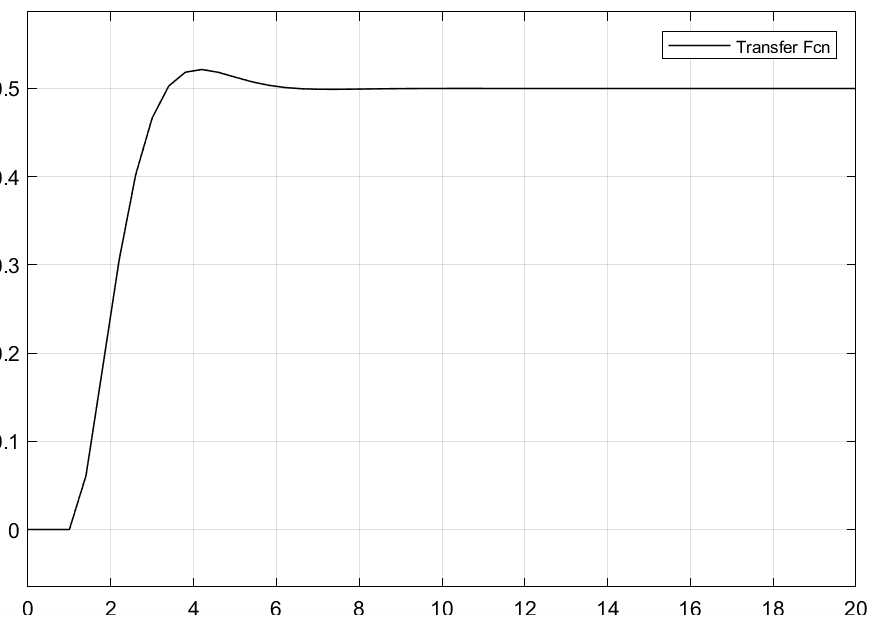
\includegraphics[scale=0.4]{function.png}
    \caption{動特性 }
\end{figure}

MATLABでシミュレーションした結果、ステップで入力したら短時間内に0.5に達し、ほぼ振動していない.決定されているのは減衰係数である.伝達関数の係数から読み取れる.\\

(3) 状態変数表現を求めよ.\\

$ x_{1}(t)=q(t),x_{2}(t)=\dot{q}(t) $とする.

\begin{equation}
\left\{
             \begin{array}{lr}
             \dot{x_{1}}(t)=x_{2}(t), & \\
             &\\
             \dot{x_{2}}(t)=v(t)-2x_{2}(t)-2x_{1}(t), & 
             \end{array}
\right.
\end{equation}

\begin{equation}
    {
\left[ \begin{array}{c}
\dot{x_{1}}(t)\\
\dot{x_{2}}(t)
\end{array}
\right ]}={
\left[ \begin{array}{cc}
0&1\\
-2&-2
\end{array}
\right ]}{
\left[ \begin{array}{c}
x_{1}(t)\\
x_{2}(t)
\end{array}
\right ]}
+{
\left[ \begin{array}{c}
0\\
1
\end{array}
\right ]}v(t)
\end{equation}

よって、状態空間表現は

\begin{equation}
\left\{
             \begin{array}{lr}
             \dot{x}(t)=Ax(t)+Bu(t), & \\
             &\\
             y(t)=Cx(t), & 
             \end{array}
\right.
\end{equation}
特に、

\begin{equation}
A={
\left[ \begin{array}{cc}
0&1\\
-2&-2
\end{array}
\right ]},B={
\left[ \begin{array}{c}
0\\
1
\end{array}
\right ]},c=[1,0]
\end{equation}


(4) 上記(3)から求められた伝達関数と上記(1)の結果が一致することを確認せよ.

\begin{equation}
G(s)=\frac{1}{s^{2}+2s+2}=C(sI-A)^{-1}B
	\end{equation}
	
	\begin{equation}
G(s)=(1,0){
\left[ \begin{array}{cc}
s & -1\\
2 & s+2
\end{array}
\right ]}^{-1}{
\left[ \begin{array}{c}
0 \\
1 
\end{array}
\right ]}
	\end{equation}
	
	\begin{equation}
=(1,0)\frac{1}{s(s+2)+2}{
\left[ \begin{array}{cc}
s+2 & 1\\
-2 & s
\end{array}
\right ]}{
\left[ \begin{array}{c}
0 \\
1 
\end{array}
\right ]}
	\end{equation}
	
	\begin{equation}
=[\frac{s+2}{s^{2}+2s+2},\frac{1}{s^{2}+2s+2}]
{
\left[ \begin{array}{c}
0 \\
1 
\end{array}
\right ]}
	\end{equation}
	
		\begin{equation}
=\frac{1}{s^{2}+2s+2}
	\end{equation}



	
	
\end{document}